%\VignetteIndexEntry{Detecting allele-specific events from ChIP-seq data}
%\VignettePackage{BaalChIP}
%\VignetteEngine{utils::Sweave}

\documentclass{article}\usepackage[]{graphicx}\usepackage[usenames,dvipsnames]{color}
%% maxwidth is the original width if it is less than linewidth
%% otherwise use linewidth (to make sure the graphics do not exceed the margin)
\makeatletter
\def\maxwidth{ %
  \ifdim\Gin@nat@width>\linewidth
    \linewidth
  \else
    \Gin@nat@width
  \fi
}
\makeatother

\definecolor{fgcolor}{rgb}{0.345, 0.345, 0.345}
\newcommand{\hlnum}[1]{\textcolor[rgb]{0.686,0.059,0.569}{#1}}%
\newcommand{\hlstr}[1]{\textcolor[rgb]{0.192,0.494,0.8}{#1}}%
\newcommand{\hlcom}[1]{\textcolor[rgb]{0.678,0.584,0.686}{\textit{#1}}}%
\newcommand{\hlopt}[1]{\textcolor[rgb]{0,0,0}{#1}}%
\newcommand{\hlstd}[1]{\textcolor[rgb]{0.345,0.345,0.345}{#1}}%
\newcommand{\hlkwa}[1]{\textcolor[rgb]{0.161,0.373,0.58}{\textbf{#1}}}%
\newcommand{\hlkwb}[1]{\textcolor[rgb]{0.69,0.353,0.396}{#1}}%
\newcommand{\hlkwc}[1]{\textcolor[rgb]{0.333,0.667,0.333}{#1}}%
\newcommand{\hlkwd}[1]{\textcolor[rgb]{0.737,0.353,0.396}{\textbf{#1}}}%

\usepackage{framed}
\makeatletter
\newenvironment{kframe}{%
 \def\at@end@of@kframe{}%
 \ifinner\ifhmode%
  \def\at@end@of@kframe{\end{minipage}}%
  \begin{minipage}{\columnwidth}%
 \fi\fi%
 \def\FrameCommand##1{\hskip\@totalleftmargin \hskip-\fboxsep
 \colorbox{shadecolor}{##1}\hskip-\fboxsep
     % There is no \\@totalrightmargin, so:
     \hskip-\linewidth \hskip-\@totalleftmargin \hskip\columnwidth}%
 \MakeFramed {\advance\hsize-\width
   \@totalleftmargin\z@ \linewidth\hsize
   \@setminipage}}%
 {\par\unskip\endMakeFramed%
 \at@end@of@kframe}
\makeatother

\definecolor{shadecolor}{rgb}{.97, .97, .97}
\definecolor{messagecolor}{rgb}{0, 0, 0}
\definecolor{warningcolor}{rgb}{1, 0, 1}
\definecolor{errorcolor}{rgb}{1, 0, 0}
\newenvironment{knitrout}{}{} % an empty environment to be redefined in TeX

\usepackage{alltt}

\RequirePackage{/Users/santia01/Library/R/3.1/library/BiocStyle/resources/latex/Bioconductor}

\AtBeginDocument{\bibliographystyle{/Users/santia01/Library/R/3.1/library/BiocStyle/resources/latex/unsrturl}}

\usepackage{float}
\IfFileExists{upquote.sty}{\usepackage{upquote}}{}
\begin{document}




\title{Detecting allele-specific events from ChIP-seq data}
\author{Ines de Santiago, Wei Liu, Ke Yuan, Bruce Ponder, Kerstin Meyer, Florian Markowetz}

\date{Edited: 2016; Compiled: \today}

\maketitle

\tableofcontents

\section{Introduction}

Allele-specific binding (ASB) measurements of transcription-factor binding from ChIP-seq data have provided important insights into the allelic effects of non-coding variants and its contribution to phenotypic diversity. However, such approaches are designed to examine the allelic imbalances in diploid samples and do not address copy number differences between the two alleles, a known phenotypical feature of cancer cells.

\Biocpkg{BaalChIP} (Bayesian Analysis of Allelic imbalances from ChIP-seq data) tests the differential read counts of the alleles at each heterozygous variant using a Bayesian framework to account for the background allele composition and other sources of bias that might influence the overall ChIP-seq read count, and takes advantage of the fact that multiple transcription factor ChIP-seq data may be available for the same variant to improve ASB detection (Figure \ref{fig:baalFramewor}).

\begin{center}
\begin{figure}[H]
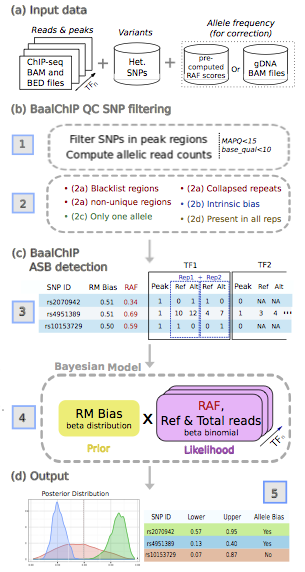
\includegraphics[scale=0.5]{baal.pdf}
\caption{Description of Baal-ChIP model frame work. (a) Input data: the reference mapping (RM) bias and reference allele frequency (RAF) have been included in the input data. The first column of peak file is the binary data used to state the calling peaks and the other columns are ChIP-seq reads count. (b) Baal-ChIP package has two modules: SNP QC filters to remove the false identified SNPs causing by technical biases and beta-binomial Bayesian model to consider RM and RAF bias. (c) Model output: the output from Baal-ChIP is posterior distribution for each SNP and user can use defined threshold to identify the SNPs with allele bias (default value for threshold is 0.5)}
\label{fig:baalFramewor}
\end{figure}
\end{center}


\section{A sample session}

This section offers a quick example of how to use \Biocpkg{BaalChIP} to identify ASB events with correction for relative allele frequency.

\subsection{Example datasets in this vignette}

The example dataset in this vignette contains ChIP-seq data obtained for two cell lines: A cancer cell-line (MCF7) and a normal cell line (GM12891). For each cell line, ChIP-seq data exists for four transcription factors and two biological replicates for each of the transcription factors. This example dataset also contains the B-allele frequency (BAF) scores obtained using Genome-Wide Human SNP Array 6.0 Affymetrix microarrays. In this example dataset, the BAF scores are used to correct the allelic read counts.

%Two example datasets are included in this vignette.
%\begin{itemize}
%\item{the first one contains ChIP-seq data obtained for two cell lines: A cancer cell-line (MCF7) and a normal cell line (GM12891). For each cell line, ChIP-seq data exists for four transcription factors and two biological replicates for each of the transcription factors. This example dataset also contains the B-allele frequency (BAF) scores obtained using Genome-Wide Human SNP Array 6.0 Affymetrix microarrays. In this example dataset, the BAF scores are used to correct the allelic read counts.}
%\item{The second dataset contains FAIRE-seq targeted sequencing for two cancer cell lines (MDA134 and T47D). For each cell line, there are two biological replicates and two replicates of targeted sequencing data for the input genomic DNA. In this example, the allelic-ratios obtained from the deeply sequenced input gDNA samples are used to correct the read counts obtained from the target enriched library.}
%\end{itemize}

Note that the example data in this vignette does not reveal real biology and was build only for demonstration purposes.

\subsection{Reading in data}

The first thing to do is to read some data.

The metadata and all files necessary for this example are available in the extra subdirectory
of the BaalChIP package directory; you can make this your working directory by entering:

\begin{knitrout}
\definecolor{shadecolor}{rgb}{0.969, 0.969, 0.969}\color{fgcolor}\begin{kframe}
\begin{alltt}
\hlkwd{library}\hlstd{(BaalChIP)}
\hlkwd{setwd}\hlstd{(}\hlkwd{system.file}\hlstd{(}\hlstr{"test"}\hlstd{,}\hlkwc{package}\hlstd{=}\hlstr{"BaalChIP"}\hlstd{))}
\end{alltt}
\end{kframe}
\end{knitrout}

The first step is to construct a \Rclass{BaalChIP} object:
\begin{knitrout}
\definecolor{shadecolor}{rgb}{0.969, 0.969, 0.969}\color{fgcolor}\begin{kframe}
\begin{alltt}
\hlstd{samplesheet} \hlkwb{<-} \hlstr{"exampleChIP.tsv"}
\hlstd{hets} \hlkwb{<-} \hlkwd{c}\hlstd{(}\hlstr{"MCF7"}\hlstd{=}\hlstr{"MCF7_hetSNP.txt"}\hlstd{,} \hlstr{"GM12891"}\hlstd{=}\hlstr{"GM12891_hetSNP.txt"}\hlstd{)}
\hlstd{res} \hlkwb{<-} \hlkwd{new}\hlstd{(}\hlstr{"BaalChIP"}\hlstd{,} \hlkwc{samplesheet}\hlstd{=samplesheet,} \hlkwc{hets}\hlstd{=hets)}
\end{alltt}
\end{kframe}
\end{knitrout}

\subsection{BaalChIP analysis}

The BaalChIP analysis can either be run with various commands (e.g. \Rfunction{alleleCounts}, \Rfunction{QCfilter}, \Rfunction{mergePerGroup}, \Rfunction{filter1allele}) one at the time, or use the function \Rfunction{BaalChIP.run} which will run a typical analysis. 

Given a new BaalChIP object, to run a BaalChIP analysis and identify allele-specific binding events, type:
\begin{knitrout}
\definecolor{shadecolor}{rgb}{0.969, 0.969, 0.969}\color{fgcolor}\begin{kframe}
\begin{alltt}
\hlstd{res} \hlkwb{<-} \hlkwd{new}\hlstd{(}\hlstr{"BaalChIP"}\hlstd{,} \hlkwc{samplesheet}\hlstd{=samplesheet,} \hlkwc{hets}\hlstd{=hets)}
\hlstd{res} \hlkwb{<-} \hlkwd{BaalChIP.run}\hlstd{(res)}
\end{alltt}
\end{kframe}
\end{knitrout}

If you wish to have more control over the input options, the same analysis above can be performed with various commands as follows:

\begin{knitrout}
\definecolor{shadecolor}{rgb}{0.969, 0.969, 0.969}\color{fgcolor}\begin{kframe}
\begin{alltt}
\hlcom{#load data}
\hlkwd{data}\hlstd{(blacklist_hg19)}
\hlkwd{data}\hlstd{(pickrell2011cov1_hg19)}
\hlkwd{data}\hlstd{(UniqueMappability50bp_hg19)}

\hlcom{#run one at the time}
\hlstd{res} \hlkwb{<-} \hlkwd{alleleCounts}\hlstd{(res,} \hlkwc{min_base_quality}\hlstd{=}\hlnum{10}\hlstd{,} \hlkwc{min_mapq}\hlstd{=}\hlnum{15}\hlstd{)}
\hlstd{res} \hlkwb{<-} \hlkwd{QCfilter}\hlstd{(res,} \hlkwc{RegionsToFilter}\hlstd{=}\hlkwd{c}\hlstd{(}\hlstr{"blacklist_hg19"}\hlstd{,} \hlstr{"pickrell2011cov1_hg19"}\hlstd{),}
                \hlkwc{RegionsToKeep}\hlstd{=}\hlstr{"UniqueMappability50bp_hg19"}\hlstd{)}
\hlstd{res} \hlkwb{<-} \hlkwd{mergePerGroup}\hlstd{(res)}
\hlstd{res} \hlkwb{<-} \hlkwd{filter1allele}\hlstd{(res)}
\hlstd{res} \hlkwb{<-} \hlkwd{getASB}\hlstd{(res,} \hlkwc{Iter}\hlstd{=}\hlnum{5000}\hlstd{,} \hlkwc{conf_level}\hlstd{=}\hlnum{0.95}\hlstd{,} \hlkwc{RMcorrection} \hlstd{=} \hlnum{TRUE}\hlstd{,} \hlkwc{RAFcorrection}\hlstd{=}\hlnum{TRUE}\hlstd{)}
\end{alltt}
\end{kframe}
\end{knitrout}

The following sections describe these steps in more detail.

\section{Notes on data entry}

\subsection{The samplesheet}

In order to run BaalChIP, one needs to generate a sample sheet describing the samples and the groups within each study. This file should be saved as a tab-delimited file. The extension of this file is not important, for example it can be \texttt{.txt} as long as it is a tab-delimited file.
A .tsv sample sheet has been included in this vignette and can be assessed as follows:

\begin{knitrout}
\definecolor{shadecolor}{rgb}{0.969, 0.969, 0.969}\color{fgcolor}\begin{kframe}
\begin{alltt}
\hlkwd{setwd}\hlstd{(}\hlkwd{system.file}\hlstd{(}\hlstr{"test"}\hlstd{,}\hlkwc{package}\hlstd{=}\hlstr{"BaalChIP"}\hlstd{))}
\hlstd{samplesheet} \hlkwb{<-} \hlkwd{read.delim}\hlstd{(}\hlstr{"exampleChIP.tsv"}\hlstd{)}
\hlstd{samplesheet}
\end{alltt}
\begin{verbatim}
##    group_name target replicate_number                       bam_name
## 1        MCF7   cFOS                1    bamFiles/MCF7_cFOS_Rep1.bam
## 2        MCF7   cFOS                2    bamFiles/MCF7_cFOS_Rep2.bam
## 3        MCF7   cMYC                1    bamFiles/MCF7_cMYC_Rep1.bam
## 4        MCF7   cMYC                2    bamFiles/MCF7_cMYC_Rep2.bam
## 5        MCF7   POL2                1    bamFiles/MCF7_POL2_Rep1.bam
## 6        MCF7   POL2                2    bamFiles/MCF7_POL2_Rep2.bam
## 7        MCF7  STAT3                1   bamFiles/MCF7_STAT3_Rep1.bam
## 8        MCF7  STAT3                2   bamFiles/MCF7_STAT3_Rep2.bam
## 9     GM12891   POL2                1 bamFiles/GM12891_POL2_Rep1.bam
## 10    GM12891   POL2                2 bamFiles/GM12891_POL2_Rep2.bam
## 11    GM12891   PAX5                1 bamFiles/GM12891_PAX5_Rep1.bam
## 12    GM12891   PAX5                2 bamFiles/GM12891_PAX5_Rep2.bam
## 13    GM12891    PU1                1  bamFiles/GM12891_PU1_Rep1.bam
## 14    GM12891    PU1                2  bamFiles/GM12891_PU1_Rep2.bam
## 15    GM12891   TAF1                1 bamFiles/GM12891_TAF1_Rep1.bam
## 16    GM12891   TAF1                2 bamFiles/GM12891_TAF1_Rep2.bam
##                     bed_name
## 1     bedFiles/MCF7_cFOS.bed
## 2     bedFiles/MCF7_cFOS.bed
## 3     bedFiles/MCF7_cMYC.bed
## 4    bedFiles//MCF7_cMYC.bed
## 5     bedFiles/MCF7_POL2.bed
## 6     bedFiles/MCF7_POL2.bed
## 7    bedFiles/MCF7_STAT3.bed
## 8    bedFiles/MCF7_STAT3.bed
## 9  bedFiles/GM12891_POL2.bed
## 10 bedFiles/GM12891_POL2.bed
## 11 bedFiles/GM12891_PAX5.bed
## 12 bedFiles/GM12891_PAX5.bed
## 13  bedFiles/GM12891_PU1.bed
## 14  bedFiles/GM12891_PU1.bed
## 15 bedFiles/GM12891_TAF1.bed
## 16 bedFiles/GM12891_TAF1.bed
\end{verbatim}
\end{kframe}
\end{knitrout}

This sample sheet details the metadata for ChIP-seq studies in MCF7 and GM12891 cell lines. For each study, ChIP-seq data exists for four transcription factors (\texttt{target}). The first column \texttt{group name} identifies the group label of each study (MCF7, GM12891). The column \texttt{replicate number} shows that there are two biological replicates for each ChIP-seq factor. The sample sheet also contains file paths to the BAM files (\texttt{bam name}) with the aligned reads and the BED files (\texttt{bed name}) with  the genomic regions of signal enrichment that the user is interested in (typically these are the ChIP-seq peaks files).   

\subsection{The hets files}

BaalChIP requires a \textquotedbl{}variant file\textquotedbl{} containing the list of heterozygous variants to be analysed. As an example, a small set of heterozygous variants for each cell line has been included in this vignette and can be assessed as follows:

\begin{knitrout}
\definecolor{shadecolor}{rgb}{0.969, 0.969, 0.969}\color{fgcolor}\begin{kframe}
\begin{alltt}
\hlkwd{setwd}\hlstd{(}\hlkwd{system.file}\hlstd{(}\hlstr{"test"}\hlstd{,}\hlkwc{package}\hlstd{=}\hlstr{"BaalChIP"}\hlstd{))}
\hlkwd{head}\hlstd{(}\hlkwd{read.delim}\hlstd{(}\hlstr{"MCF7_hetSNP.txt"}\hlstd{))}
\end{alltt}
\begin{verbatim}
##           ID CHROM       POS REF ALT       RAF
## 1 rs10169169  chr2 191412889   T   G 0.4870296
## 2  rs1021813  chr3  59413060   T   C 0.4689580
## 3  rs1025641 chr10 128307192   T   C 0.4077530
## 4 rs10444404 chr12  15114751   T   G 0.5195654
## 5  rs1048347 chr10 124096061   A   C 0.4852518
## 6 rs10495062  chr1 217804955   T   C 0.3654244
\end{verbatim}
\end{kframe}
\end{knitrout}

The information in the variant file should include an \texttt{ID} column with a unique identifier string per variant, the (1-based) genomic coordinates \texttt{CHROM, POS}, and the A,C,G,T bases for the reference \texttt{REF} and the non-reference alternate \texttt{ALT} allele. 

The final column \texttt{RAF} consists of a value ranging from 0 to 1 for each variant denoting the relative allele frequency. A value between 0.5 and 1 denotes a bias to the reference allele, and a value between 0 and 0.5 a bias to the alternate allele. This column is optional, and will not be necessary if we ask BaalChIP to calculate the RAF values from the input gDNA libraries. If both gDNA and RAF values are missing BaalChIP will still run but will not correct for relative allele frequency (copy-number) bias.

%\subsection{the gDNA files}

%These argument is an optional list of input genomic DNA samples.
%Continue here

\section{Constructing a BaalChIP object}

The first step is to generate a BaalChIP object. The function \texttt{new} accepts a samplesheet and a named vector containing the filenames for the variant files to be used. The names in the vector should correspond to \texttt{group\_name} strings in the \texttt{.csv} samplesheet, in this case it should be \textquotedbl{}MCF7\textquotedbl{} and \textquotedbl{}GM12891\textquotedbl{}.

\begin{knitrout}
\definecolor{shadecolor}{rgb}{0.969, 0.969, 0.969}\color{fgcolor}\begin{kframe}
\begin{alltt}
\hlstd{samplesheet} \hlkwb{<-} \hlstr{"example.tsv"}
\hlstd{hets} \hlkwb{<-} \hlkwd{c}\hlstd{(}\hlstr{"MCF7"}\hlstd{=}\hlstr{"MCF7_hetSNP.txt"}\hlstd{,} \hlstr{"GM12891"}\hlstd{=}\hlstr{"GM12891_hetSNP.txt"}\hlstd{)}
\hlstd{res} \hlkwb{<-} \hlkwd{new}\hlstd{(}\hlstr{"BaalChIP"}\hlstd{,} \hlkwc{samplesheet}\hlstd{=samplesheet,} \hlkwc{hets}\hlstd{=hets)}
\end{alltt}
\end{kframe}
\end{knitrout}

the samplesheet is saved in the \texttt{samples} slot of a BaalChIP object:

\begin{knitrout}
\definecolor{shadecolor}{rgb}{0.969, 0.969, 0.969}\color{fgcolor}\begin{kframe}
\begin{alltt}
\hlstd{res}\hlopt{@}\hlkwc{samples}
\end{alltt}
\end{kframe}
\end{knitrout}

\subsection{Obtaining allele-specific counts for BAM files}

The next step is to compute, for each variant the number of reads carrying the reference (REF) and alternative (ALT) alleles. The \Rfunction{alleleCounts} function will read and scan all BAM files  within the \texttt{samples} slot of a BaalChIP object and compute the read coverage at each allele. Allele counts are computed using the \Rfunction{pileup} function and the \texttt{PileupParam} constructor of the \Biocpkg{Rsamtools} package (Morgan et al., 2016). 
For each BAM file, it will only consider heterozygous SNPs overlapping the genomic regions in the 
corresponding BED files. Two arguments can be manipulated by the user: the \texttt{min\_mapq} refers to the minimum \textquotedbl{}MAPQ\textquotedbl{} value for an alignment to be included in pileup (default is 15); and the \texttt{min\_base\_quality} which refers to the minimum \textquotedbl{}QUAL\textquotedbl{} value for each nucleotide in an alignment (default is 10).

\begin{knitrout}
\definecolor{shadecolor}{rgb}{0.969, 0.969, 0.969}\color{fgcolor}\begin{kframe}
\begin{alltt}
\hlstd{res} \hlkwb{<-} \hlkwd{alleleCounts}\hlstd{(res,} \hlkwc{min_base_quality}\hlstd{=}\hlnum{10}\hlstd{,} \hlkwc{min_mapq}\hlstd{=}\hlnum{15}\hlstd{)}
\hlstd{res}
\end{alltt}
\end{kframe}
\end{knitrout}


\subsection{QCfilter: A filter to exclude SNPs in regions of known problematic read alignment}

After computing the read counts per allele, the next step in the BaalChIP pipeline is an extensive quality control step to consider technical biases that may contribute to the false identification of regulatory SNPs.

The function \Rfunction{QCfilter} is used to excluded sites susceptible to allelic mapping bias in regions of known problematic read alignment (Pickrell et al., 2011; Consortium, 2012). This function accepts two arguments: \textquotedbl{}RegionsToFilter\textquotedbl{} with the genomic regions to be excluded, and \textquotedbl{}RegionsToKeep\textquotedbl{} with the genomic regions to be kept. 

Three datafiles are included with BaalChIP package for the human genome: 

(1) blacklisted regions downloaded from the UCSC Genome Browser (mappability track; release 3, October 2011; thewgEncodeDacMapabilityConsensusExcludable and wgEncodeDukeMapabilityRegionsExcludable tables), (2) non-unique regions selected from DUKE uniqueness mappability track of the UCSC genome browser (release 3, October 2011; wgEncodeCrgMapabilityAlign50mer table), and (3) collapsed repeat regions downloaded from Pickrell et al., 2010 at the 0.1\% threshold. 

\begin{knitrout}
\definecolor{shadecolor}{rgb}{0.969, 0.969, 0.969}\color{fgcolor}\begin{kframe}
\begin{alltt}
\hlkwd{data}\hlstd{(blacklist_hg19)}
\hlkwd{data}\hlstd{(pickrell2011cov1_hg19)}
\hlkwd{data}\hlstd{(UniqueMappability50bp_hg19)}

\hlstd{res} \hlkwb{<-} \hlkwd{QCfilter}\hlstd{(res,}
                \hlkwc{RegionsToFilter}\hlstd{=}\hlkwd{list}\hlstd{(}\hlstr{"blacklist"}\hlstd{=blacklist_hg19,} \hlstr{"highcoverage"}\hlstd{=pickrell2011cov1_hg19),}
                \hlkwc{RegionsToKeep}\hlstd{=}\hlkwd{list}\hlstd{(}\hlstr{"UniqueMappability"}\hlstd{=UniqueMappability50bp_hg19))}
\hlstd{res} \hlkwb{<-} \hlkwd{mergePerGroup}\hlstd{(res)}
\hlstd{res} \hlkwb{<-} \hlkwd{filter1allele}\hlstd{(res)}
\end{alltt}
\end{kframe}
\end{knitrout}

%\subsection{filtIntBias: A simulation-based filtering to exclude SNPs with intrinsic bias}
%The function \Rfunction{filtIntBias} can be used to apply a simulation-based filtering to exclude SNPs with intrinsic bias to one of the alleles (Degner et al., 2009; Pickrell et al., 2010)

%\subsection{Merge allele counts per group}
%The function \Rfunction{mergePerGroup} is used to considered only SNPs that pass all filters in all replicated samples; 
%The function \Rfunction{filter1allele} is used to exclude variants where only one allele was observed after pooling ChIP-seq reads from all examined samples, indicating that those variants are possibly homozygous (Lappalainen et al., 2013; Kilpinen et al., 2013). 

%\section{An example with ENCODE dataset}


\section{Summarizing and plotting QC data}



\begin{knitrout}
\definecolor{shadecolor}{rgb}{0.969, 0.969, 0.969}\color{fgcolor}\begin{kframe}
\begin{alltt}
\hlkwd{plotQC}\hlstd{(res,} \hlstr{"barplot_per_group"}\hlstd{)}
\end{alltt}
\end{kframe}

{\centering 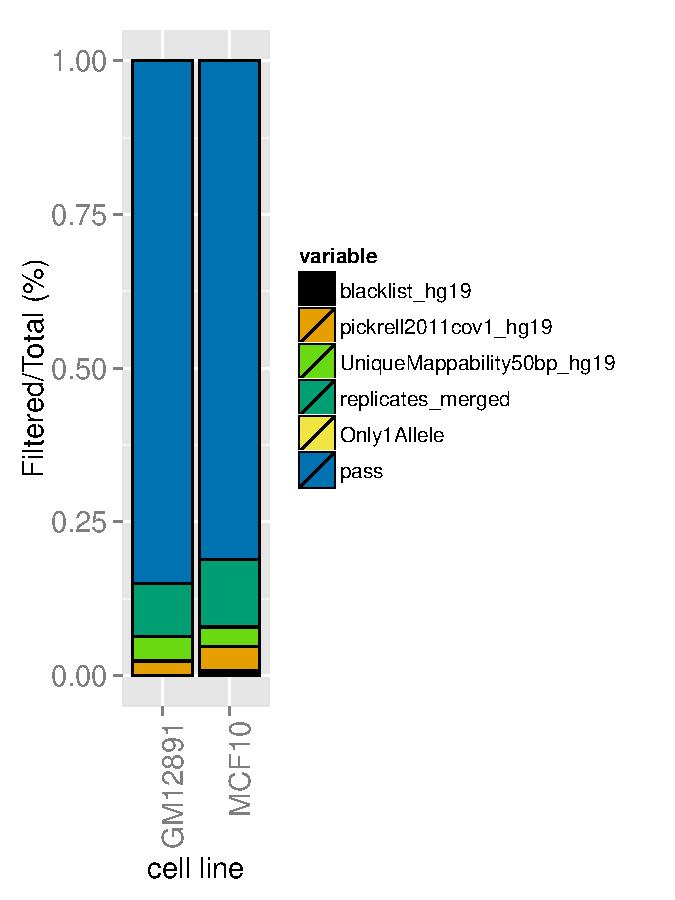
\includegraphics[width=\maxwidth]{figure/QCplots-1} 

}


\begin{kframe}\begin{alltt}
\hlkwd{plotQC}\hlstd{(res,} \hlstr{"boxplot_per_filter"}\hlstd{)}
\end{alltt}
\end{kframe}

{\centering 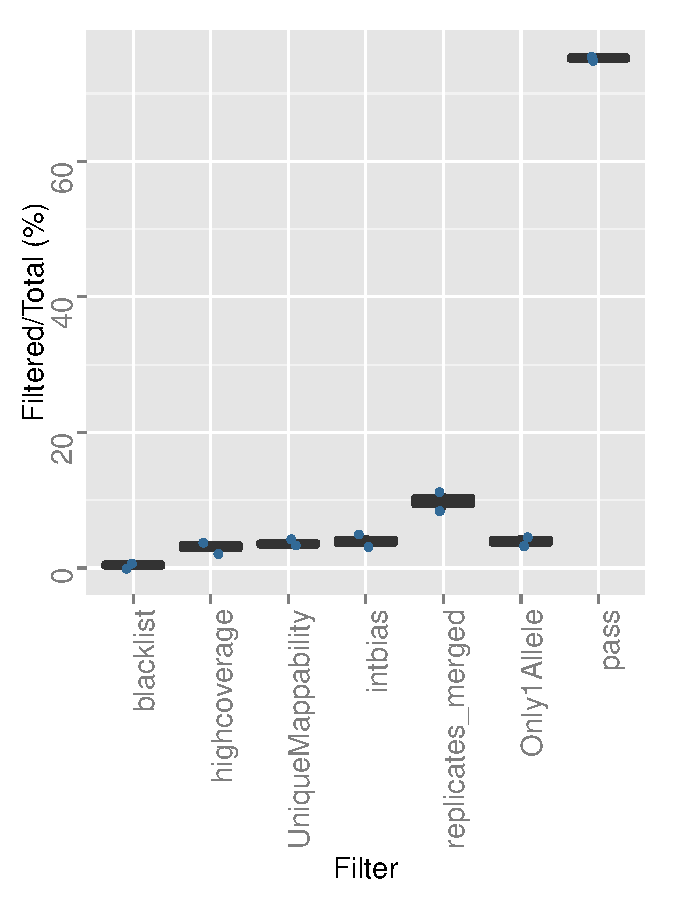
\includegraphics[width=\maxwidth]{figure/QCplots-2} 

}


\begin{kframe}\begin{alltt}
\hlkwd{plotQC}\hlstd{(res,} \hlstr{"overall_pie"}\hlstd{)}
\end{alltt}
\end{kframe}

{\centering 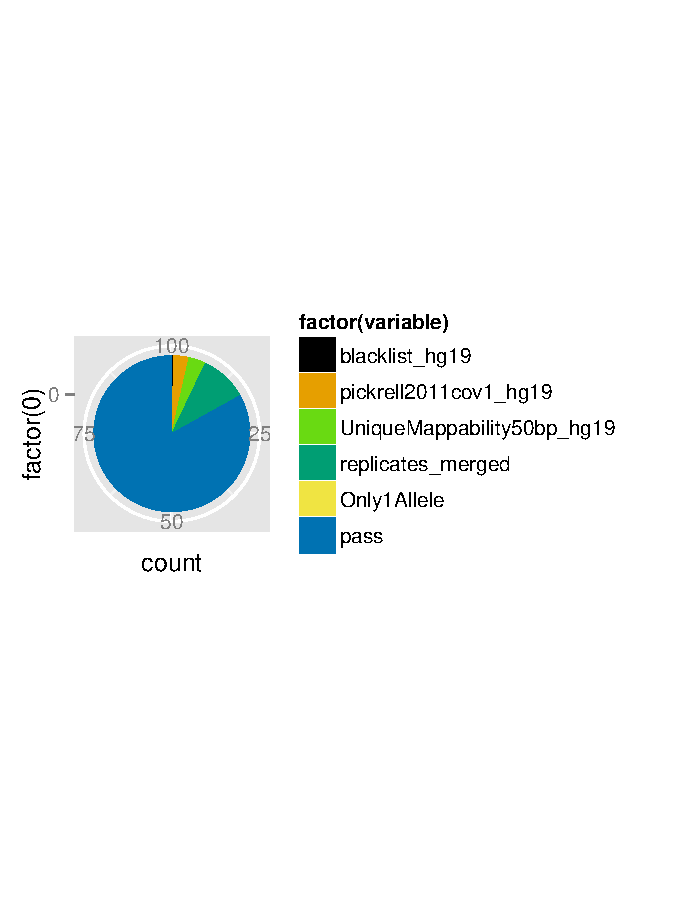
\includegraphics[width=\maxwidth]{figure/QCplots-3} 

}


\begin{kframe}\begin{alltt}
\hlkwd{summaryQC}\hlstd{(res)}
\end{alltt}
\begin{verbatim}
## $filtering_stats
##         blacklist highcoverage UniqueMappability intbias replicates_merged Only1Allele
## MCF7            1            5                 4       4                14           4
## GM12891         0            3                 5       6                11           6
##         pass
## MCF7      95
## GM12891   96
## 
## $average_stats
##            variable value.mean       perc
## 1         blacklist        0.5  0.3937008
## 2      highcoverage        4.0  3.1496063
## 3 UniqueMappability        4.5  3.5433071
## 4           intbias        5.0  3.9370079
## 5 replicates_merged       12.5  9.8425197
## 6       Only1Allele        5.0  3.9370079
## 7              pass       95.5 75.1968504
\end{verbatim}
\end{kframe}
\end{knitrout}

The function BaalChIP.report outputs a table with all assayed variants and with additional information about their ASB status:

\begin{knitrout}
\definecolor{shadecolor}{rgb}{0.969, 0.969, 0.969}\color{fgcolor}\begin{kframe}
\begin{alltt}
\hlstd{result} \hlkwb{<-} \hlkwd{BaalChIP.report}\hlstd{(res)}
\hlkwd{head}\hlstd{(result[[}\hlstr{"MCF7"}\hlstd{]])}
\end{alltt}
\begin{verbatim}
##           ID CHROM       POS REF ALT REF.counts ALT.counts Total.counts         AR
## 1 rs10169169  chr2 191412889   T   G          4         19           23 0.17391304
## 2  rs1021813  chr3  59413060   T   C          3         18           21 0.14285714
## 3 rs10444404 chr12  15114751   T   G          1         14           15 0.06666667
## 4 rs10495062  chr1 217804955   T   C          2         13           15 0.13333333
## 5 rs10502400 chr18  10353940   A   G          4         17           21 0.19047619
## 6 rs10512030  chr9  76484346   T   C          1         15           16 0.06250000
##      RMbias       RAF Bayes_lower Bayes_upper Corrected.AR isASB
## 1 0.4946235 0.4870296  0.09275682   0.3900729    0.2414148  TRUE
## 2 0.4946235 0.4689580  0.07535283   0.3808823    0.2281176  TRUE
## 3 0.4946235 0.5195654  0.02347753   0.2964224    0.1599500  TRUE
## 4 0.4946235 0.3654244  0.08792807   0.5073374    0.2976327 FALSE
## 5 0.4946235 0.4670719  0.10302328   0.4302656    0.2666444 FALSE
## 6 0.4946235 0.4328198  0.02752114   0.3427208    0.1851210  TRUE
\end{verbatim}
\end{kframe}
\end{knitrout}

%\subsubsection{Identifying allele-specific binding events with RAF copy-number correction}

%<<asb1, eval=FALSE>>=
%res1 <- getASB(res, Iter=5000, conf_level=0.95, RAFcorrection=TRUE)
%result_Corrected <- BaalChIP.report(res1)
%summaryASB(res1)
%@

%\subsubsection{Identifying allele-specific binding events with without RAF copy-number correction}

%<<asb2, eval=FALSE>>=
%res2 <- getASB(res, Iter=5000, conf_level=0.95, RAFcorrection=FALSE)
%result_NOTcorrected <- BaalChIP.report(res2)
%summaryASB(res2)
%@

%\section{An example with genomic DNA files}


\section*{Acknowledgements}
We thank Thomas Carroll and Gordon Brown for suggestions and advice about ChIP-seq data analysis, and the ENCODE Consortium and the ENCODE production laboratories for generating the datasets used in this study. We thank the \href{https://give.bcrfcure.org/checkout/donation?eid=31404&_ga=1.141086386.1225939115.1465824174}{"Breast Cancer Research Foundation"} for financial support of this work.


\section*{Session Info}
\begin{kframe}
\begin{alltt}
\hlkwd{toLatex}\hlstd{(}\hlkwd{sessionInfo}\hlstd{())}
\end{alltt}
\end{kframe}\begin{itemize}\raggedright
  \item R version 3.1.3 (2015-03-09), \verb|x86_64-apple-darwin10.8.0|
  \item Locale: \verb|en_GB.UTF-8/en_GB.UTF-8/en_GB.UTF-8/C/en_GB.UTF-8/en_GB.UTF-8|
  \item Base packages: base, datasets, graphics, grDevices, methods, parallel,
    stats, stats4, utils
  \item Other packages: BaalChIP~0.1.0, BiocGenerics~0.12.1, Biostrings~2.34.1,
    doBy~4.5-13, GenomeInfoDb~1.2.5, GenomicAlignments~1.2.2,
    GenomicRanges~1.18.4, ggplot2~1.0.1, IRanges~2.0.1, knitr~1.10.5,
    reshape2~1.4.1, Rsamtools~1.18.3, S4Vectors~0.4.0, survival~2.38-1,
    XVector~0.6.0
  \item Loaded via a namespace (and not attached): base64enc~0.1-2,
    BatchJobs~1.6, BBmisc~1.9, BiocParallel~1.0.3, BiocStyle~1.4.1,
    bitops~1.0-6, brew~1.0-6, checkmate~1.5.2, codetools~0.2-11,
    colorspace~1.2-6, DBI~0.3.1, digest~0.6.8, evaluate~0.7, fail~1.2,
    foreach~1.4.2, formatR~1.2, grid~3.1.3, gtable~0.1.2, highr~0.5,
    iterators~1.0.7, labeling~0.3, lattice~0.20-31, magrittr~1.5, MASS~7.3-40,
    Matrix~1.2-0, munsell~0.4.2, plyr~1.8.2, proto~0.3-10, Rcpp~0.11.6,
    RSQLite~1.0.0, scales~0.2.4, sendmailR~1.2-1, splines~3.1.3, stringi~0.4-1,
    stringr~1.0.0, tools~3.1.3, zlibbioc~1.12.0
\end{itemize}


\section*{References}

Consortium EP. 2012. An integrated encyclopedia of dna elements in the human genome. Nature 489: 57-74.

Degner JF, Marioni JC, Pai AA, Pickrell JK, Nkadori E, Gilad Y, and Pritchard JK. 2009. Effect of read-mapping biases on detecting allele-specific expression from rna-sequencing data. Bioinformatics 25: 3207-3212.

Morgan M, Pages H, Obenchain V and Hayden N (2016). Rsamtools: Binary alignment (BAM), FASTA, variant call (BCF), and tabix file import. R package version 1.24.0, \href{http://bioconductor.org/packages/release/bioc/html/Rsamtools.html}{http://bioconductor.org/packages/release/bioc/html/Rsamtools.html}. 

Pickrell JK, Marioni JC, Pai AA, Degner JF, Engelhardt BE, Nkadori E, Veyrieras JB, Stephens M, Gilad Y, and Pritchard JK. 2010. Understanding mechanisms underlying human gene expression variation with rna sequencing. Nature 464: 768-772.

R Core Team. 2014. R: A Language and Environment for Statistical Computing. R Foundation for Statistical Computing, Vienna, Austria.

\end{document}
